\chapter{Desarrollo teórico}
En este capítulo estableceremos la base matemática del proyecto. Principalmente nos basaremos en 
los libros \textit{Advanced Data Analysis
from an Elementary Point of View} \cite{ada} y \textit{Probabilistic Networks for Practitioners — A
Guide to Construction and Analysis of Bayesian
Networks and Influence Diagrams} \cite{pgm}, junto con el capítulo \textit{An overview of the representation and 
discovery of causal relationships using bayesian networks} \cite{cooper}.

\section{Fundamentos de redes}
Las redes probabilísticas son modelos gráficos de interacciones (causales) entre una
conjunto de variables, donde las variables se representan como vértices (también nodos)
de un gráfico y las interacciones (dependencias directas) como aristas dirigidas (también
enlaces y arcos) entre los vértices. Cualquier par de vértices no conectados indican 
independencia (condicional) entre las variables representadas
por estos vértices en circunstancias particulares que se pueden leer fácilmente desde el
grafico. Por lo tanto, las redes probabilísticas capturan un conjunto de dependencia (condicional)
y propiedades de independencia asociadas con las variables representadas en la red.

Los grafos han demostrado ser un lenguaje muy intuitivo para representar
tales declaraciones de dependencia e independencia, y por lo tanto proporcionan un excelente
lenguaje para comunicar y discutir las relaciones entre las 
variables del dominio del problema, las cuales se pueden representar de forma muy compacta 
mediante grafos dirigidos acíclicos (DAG).

Las redes probabilísticas pueden verse como representaciones compactas de reglas de causa-efecto "difusas" 
que, contrariamente a los sistemas normales basados en reglas, son capables de realizar tanto razonamiento 
deductivo y abductivo, como intercausal. El razonamiento deductivo o causal
sigue la dirección de los vínculos causales que hay entre las variables de un modelo; por ejemplo, al saber
que un paciente sufre de angina podemos concluir con alta probabilidad que
el paciente tiene fiebre y dolor de garganta. Por otro lado, el razonamiento abductivo o diagnóstico 
va en contra de la dirección de los nexos causales; por ejemplo, observar
que un paciente tiene dolor de garganta proporciona evidencia de que anginas es un diagnóstico correcto.

Sin embargo, la propiedad que distingue a la inferencia en redes probabilísticas
de otros paradigmas de razonamiento automático es su capacidad para hacer razonamientos intercausales: 
obtener evidencia que apoye una sola hipótesis o un subconjunto de
hipótesis conduce a la disminución de la creencia en las otras con las que compiten y para las que no se 
han encontrado unas bases que las soporten. Por ejemplo, hay un gran número de posibles causas por las que un coche
puede no arrancar, entre ellas falta de combustible. Observar que el indicador de combustible indica que no hay combustible
proporciona una fuerte evidencia de que la falta de combustible es la causa del problema, a la vez que la
la creencia en otras causas posibles disminuye sustancialmente. La capacidad de las redes probabilísticas para automáticamente
realizar tal inferencia intercausal de manera adecuada es una contribución clave a su poder de razonamiento.

A menudo, la parte gráfica de una red probabilística se conoce como aspecto cualitativo, mientras que la 
parte probabilística y numérica, como su aspecto cuantitativo. Nos dedicaremos primeramente al aspecto 
cualitativo de las redes probabilísticas.

\subsection{Fundamentos de grafos}
Un grafo es un par $G = (V, E)$, donde $V$ es un conjunto finito de vértices distinguibles y 
$E \subseteq V \times V$ es un conjunto de aristas. Un par ordenado $(u, v) \in E$ denota un borde dirigido
del vértice $u$ al vértice $v$, y se dice que $u$ es padre de $v$ y $v$ hijo de $u$.
El conjunto de padres e hijos de un vértice $v$ se denotará por $pa(v)$ y $ch(v)$, respectivamente.
Los bordes dirigidos se representarán como flechas, y los bordes no dirigidos como líneas. 

\begin{figure}[h!]
    \centering
     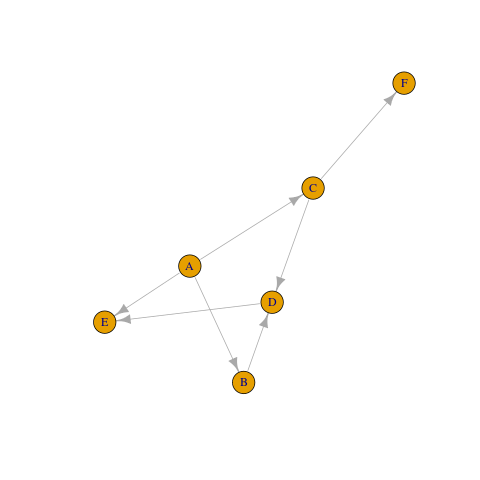
\includegraphics[width=\textwidth]{./img/dag.png}
     \caption{Ejemplo de grafo dirigido acíclico (DAG)}
     \label{img:dag1}
    \end{figure}

Una forma relativamente natural de ver un partido de fútbol es como una secuencia de 
pases entre jugadores e intercepciones, que terminan en una resolución. 

Si $E$ no contiene bordes no dirigidos, entonces $G$ es un grafo dirigido, y si $E$ no 
contiene bordes dirigidos, entonces es un grafo no dirigido. Un camino $ \langle v_{1},...,v_{n} \rangle $ 
es una secuencia de vértices distinguidos tales que $u \rarrow v$, $v \rarrow u$ o $u - v$ para 
cada $i= 1,..., n-1$. 
La longitud del camino es $n-1$. El camino es dirigido si $v_{i} \rarrow v_{i+1}$ para cada $i= 1,..., n-1$; $v_{i}$ es 
por tanto un ancestro de $v_{j}$ y $v_{j}$ es un descendiente de $v_{i}$ para cada $j > i$. El conjunto de ancestros y 
descendientes de $v$ se denota $an(v)$ y $de(v)$, respectivamente.

Un grafo $G= (V, E)$ está conectado si para cada par ${u, v} \subseteq V$ hay un camino $ \langle u,...,v \rangle$ en $G$. Un 
grafo conectado es un árbol si para cualquier par ${u,v} \subseteq V$ hay un único camino $\langle u,...,v \rangle$ en $G$. Un ciclo 
es un camino, $\langle u,...,v \rangle$, de longitud mayor que dos (excepto el caso $v_{1} = v_{n}$); un grafo dirigido sin ciclos dirigidos 
es el ya mencionado DAG. 

\subsection{Modelos gráficos}
En un nivel estructural o cualitativo, los modelos de redes probabilísticas son grafos cuyos vértices 
representan variables y funciones, y los bordes representan distintos tipos de relaciones entre ellas. 

\subsubsection{Variables}
Una variable representa un conjunto exhaustivo de eventos mutuamente excluyentes, conocidos como dominio de la variable. Estos 
eventos también se pueden llamar estados, niveles, valores, elecciones o opciones. El dominio de una variable puede ser discreto o 
contínuo; los dominios discretos son siempre finitos. Usaremos letras mayúsculas para denotar variables o conjuntos de variables, 
y letras minúsculas para sus valores. Consecuentemente, $X = x$ puede denotar el hecho de que la variable $X$ toma el valor $x$ o que 
el conjunto de variables $X = (X_{1},...,X_{n})$ toma el vector de valores $x = (x_{1},...,x_{n})$. Por $dom(X)= (x_{1},...,x_{||X||})$ 
denotaremos el dominio de $X$, donde $||X|| = |dom(X)|$ es el número de posibles valores de $X$. Si $X = (X_{1},...,X_{n})$, entonces $dom(X)$ 
es el producto cartesiano sobre los dominios de las variables en $X$, $$dom(X)=dom(X_{1})\times ... \times dom(X_{n})$$, y por lo tanto $||X|| = \prod_i ||X_{i}||$. 
Para dos (conjuntos de) variables $X$ e $Y$ escribiremos $dom(X \union Y)$ o $dom(X,Y)$ para denotar $dom(X) \times dom(Y)$.

Básicamente hay dos categorías de variables: aquellas representando eventos aleatorios y aquellas que representan elecciones bajo el 
control de algún agente externo (normalmente humano). Consecuentemente, la primera categoría de variables se denomina variables aleatorias y la segunda 
variables de decisión.

Para modelos que no contienen variables de decisión o funciones (como las redes bayesianas), la noción de variable y vértice (o nodo) son usadas 
indistintamente.  

\subsection{Causalidad}
La causalidad tiene un papel muy importante en el proceso de construcción de modelos de redes probabilísticas. Una variable $X$ se dice que es 
una causa directa de $Y$ si al establecer el valor de $X$ por la fuerza, el valor de $Y$ cambia y no hay otra variable $Z$ que sea causa directa de 
$Y$ tal que $X$ es causa directa de $Z$. Para representar correctamente las relaciones de dependencia e independencia que existen en un conjunto de variables 
del dominio de un problema, es muy útil tener las relaciones de causalidad que hay entre las variables representadas como enlaces dirigidos desde las causas 
a los efectos. Esto es, si $X$ es una causa directa de $Y$, tenemos que asegurarnos de añadir un enlace desde $X$ a $Y$. 

En las siguientes subsecciones discutiremos cada uno de las posibles formas de conexión que pueden aparecer en una red.

\section{Probabilidades} 
% issue #61
\section{Redes probabilísticas}
%¿Por qué nos interesa esto? ¿Qué vamos a hacer con ellas?
%¿Qué tienen que ver con los grafos? O igual simplemente haz una referencia.
Las redes probabilísticas son modelos gráficos de interacciones (causales) entre una
conjunto de variables, donde las variables se representan como vértices (también: nodos)
de un gráfico y las interacciones (dependencias directas) como aristas dirigidas (también:
enlaces y arcos) entre los vértices. Cualquier par de vértices no conectados indican 
independencia (condicional) entre las variables representadas
por estos vértices en circunstancias particulares que se pueden leer fácilmente desde el
grafico. Por lo tanto, las redes probabilísticas capturan un conjunto de dependencia (condicional)
y propiedades de independencia asociadas con las variables representadas en el
la red.

Los grafos han demostrado ser un lenguaje muy intuitivo para representar
tales declaraciones de dependencia e independencia, y por lo tanto proporcionan una excelente
lenguaje para comunicar y discutir las relaciones entre las 
variables del dominio del problema, las cuales se pueden representar de forma muy compacta 
mediante grafos dirigidos acíclicos (DAG).

Las redes probabilísticas pueden verse como representaciones compactas de reglas de causa-efecto "difusas" 
que, contrariamente a los sistemas normales basados en reglas, son capables de realizar tanto razonamiento 
deductivo y abductivo, como intercausal. El razonamiento deductivo o causal
sigue la dirección de los vínculos causales que hay entre las variables de un modelo; por ejemplo, al saber
que un paciente sufre de angina podemos concluir con alta probabilidad que
el paciente tiene fiebre y dolor de garganta. Por otro lado, el razonamiento abductivo o diagnóstico 
va en contra de la dirección de los nexos causales; por ejemplo, observar
que un paciente tiene dolor de garganta proporciona evidencia de que anginas es un diagnóstico correcto.

% de qué hipótesis estamos hablando en este caso?
Sin embargo, la propiedad que distingue a la inferencia en redes probabilísticas
de otros paradigmas de razonamiento automático es su capacidad para hacer razonamientos intercausales: 
obtener evidencia que apoye una sola hipótesis (o un subconjunto de
hipótesis) conduce a la disminución de la creencia en las otras con las que compiten y para las que no se 
han encontrado unas bases que las soporten. 

\section{Redes causales}

\section{Introducción a las redes bayesianas}
Las redes bayesianas nos ayudan a modelar y entender las muchas variables que informan nuestro proceso de 
toma de decisiones. Las decisiones más complejas están normalmente basadas en una multitud de factores o 
variables. Por ejemplo, para el presidente de un equipo de fútbol \ref{hu:presidente}, podemos 
mapear la decisión que tiene que tomar y las diferentes variables usando 
una red bayesiana, esto es, un modelo gráfico que captura la relación entre variables que están bajo 
supuestos de causalidad o influencia \cite{things-to-know-BN}.

Básicamente entonces, \textbf{una red bayesiana es un diagrama que 
usa flechas o arcos dirigidos para mostrar cómo distintos factores, representados por nodos elípticos, se 
influencian los unos a los otros.} Cada nodo viene con una tabla de probabilidades condicionadas, la cual refleja las 
posibilidades de varios desenlaces, provenientes de las influencias que le afectan directamente. Una vez 
la estructura del grafo y dicha tabla han sido definidas, hay algoritmos estándar que 
calculan los estados de las variables desconocidas basándose en los estados de las variables conocidas en el
modelo \cite{learning-algorithms-BN-comparison}, \cite{BN-achilles-heel}, \cite{different-algorithmic-schemes}.

Una de las razones por las que las redes bayesianas son tan potentes es que pueden realizar inferencias 
tanto predictivas como diagnósticas. Por ejemplo, podemos por un lado predecir la posición en la liga de un equipo para 
un valor dado (observación) de rendimiento, y por otro ingresar un estado de posición en la 
liga como observación para examinar qué nivel de desempeño del equipo podría explicarla. Estos algoritmos estándar son
llamados algoritmos de "propagación bayesiana" \cite{Cano2004}, \cite{more-algorithms}, \cite{back-prop} porque se basan en el teorema de Bayes, en el que la 
probabilidad de una variable desconocida se actualiza después de que se obtenga evidencia relevante para esa variable \cite{prop-alg}.

En una red bayesiana, la inferencia probabilística está determinada por los siguientes tipos de causalidad: 
\begin{itemize}
    \item \textbf{Cadena causal}: describe variables que tienen un efecto dominó las unas sobre las otras. Por ejemplo, \textit{cambios en la calidad de 
    los jugadores} tiene impacto sobre el \textit{desempeño del equipo} que a su vez influencia la \textit{posición en la liga}. 
    Esto quiere decir que la \textit{posición en la liga} es independiente de los \textit{cambios en la calidad de los jugadores} una vez conocemos el \texit{desempeño del equipo}.\\
    cambios en la calidad de los jugadores $\rightarrow$ Desempeño del equipo $\rightarrow$ Posición en la liga
    \item \textbf{Efecto común}: ocurre cuando dos variables diferentes, tales como \textit{fichajes} y \textit{jugadores vendidos}, tienen influencia sobre una tercera variable tal como 
    \textit{gasto neto en transferencias}. Esto significa que \textit{jugadores vendidos} depende de \textit{fichajes} una vez que conocemos el \textit{gasto neto en transferencias}.\\
    Fichajes $\rightarrow$ Gasto neto en transferencias $\leftarrow$ Jugadores vendidos    
    \item \textbf{Causa común}: tiene lugar cuando dos variables distintas, tales como \textit{posición en la liga} y \textit{asistencia}, se ven influenciados por la misma variable, tal 
    como \textit{desempeño del equipo}. Ello significa que \textit{asistencia} es independiente de \textit{posición en la liga} una vez conocemos \textit{desempeño del equipo}.\\
    Posición en la liga $\leftarrow$ Desempeño del equipo $\rightarrow$ Asistencia
\end{itemize}

Estas son pues las tres clases de causalidades que producen redes bayesianas.
\section{Resolución de redes probabilísticas}

